% To je predloga za poročila o domačih nalogah pri predmetih, katerih
% nosilec je Blaž Zupan. Seveda lahko tudi dodaš kakšen nov, zanimiv
% in uporaben element, ki ga v tej predlogi (še) ni. Več o LaTeX-u izveš na
% spletu, na primer na http://tobi.oetiker.ch/lshort/lshort.pdf.
%
% To predlogo lahko spremeniš v PDF dokument s pomočjo programa
% pdflatex, ki je del standardne instalacije LaTeX programov.

\documentclass[a4paper,11pt]{article}
\usepackage{a4wide}
\usepackage{fullpage}
\usepackage[utf8x]{inputenc}
\usepackage[slovene]{babel}
\selectlanguage{slovene}
\usepackage[toc,page]{appendix}
\usepackage[pdftex]{graphicx} % za slike
\usepackage{setspace}
\usepackage{color}
\definecolor{light-gray}{gray}{0.95}
\usepackage{listings} % za vključevanje kode
\usepackage{hyperref}
\usepackage{float}
\renewcommand{\baselinestretch}{1.2} % za boljšo berljivost večji razmak
\renewcommand{\appendixpagename}{Priloge}

\lstset{ % nastavitve za izpis kode, sem lahko tudi kaj dodaš/spremeniš
language=Python,
basicstyle=\footnotesize,
basicstyle=\ttfamily\footnotesize\setstretch{1},
backgroundcolor=\color{light-gray},
}

\title{Prva domača naloga}
\author{Anže Pečar (63060257)}
\date{\today}

\begin{document}

\maketitle

\section{Uvod}
\section{Metode}
\section{Rezultati}
\subsection{Grafi}
\begin{figure}[H]
\begin{center}
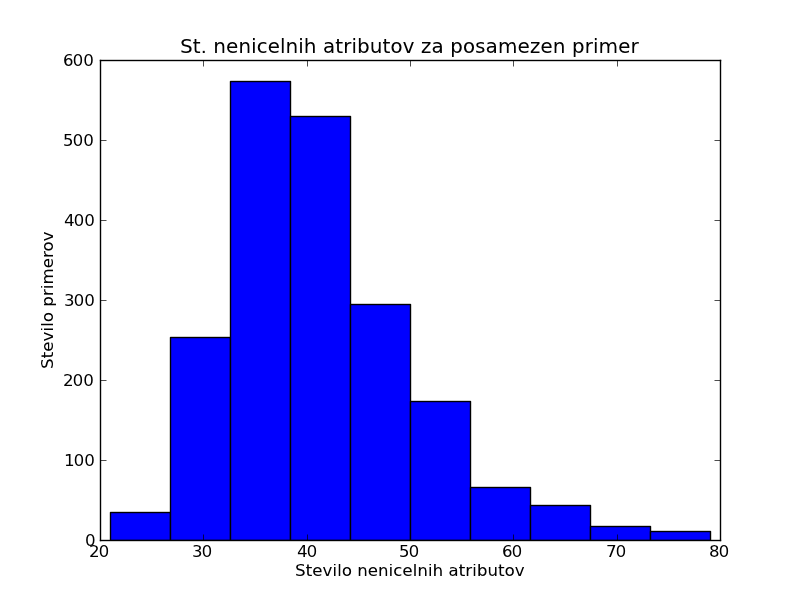
\includegraphics[scale=0.5]{examples.png}
\caption{Prikaz atributov, ki imajo vrednost različno od 0 za posamezen primer}
\label{primeri}
\end{center}
\end{figure}
\subsection{Hitrost izvajanja}
10 permutacij:
\begin{verbatim}
real	8m20.437s
user	8m18.875s
sys	0m0.628s
\end{verbatim}
100 permutacij:
\begin{verbatim}
real	73m46.716s
user	73m36.088s
sys	0m2.380s

\end{verbatim}
500 permutacij:
\begin{verbatim}

\end{verbatim}

%\begin{figure}[H]
%\begin{center}
%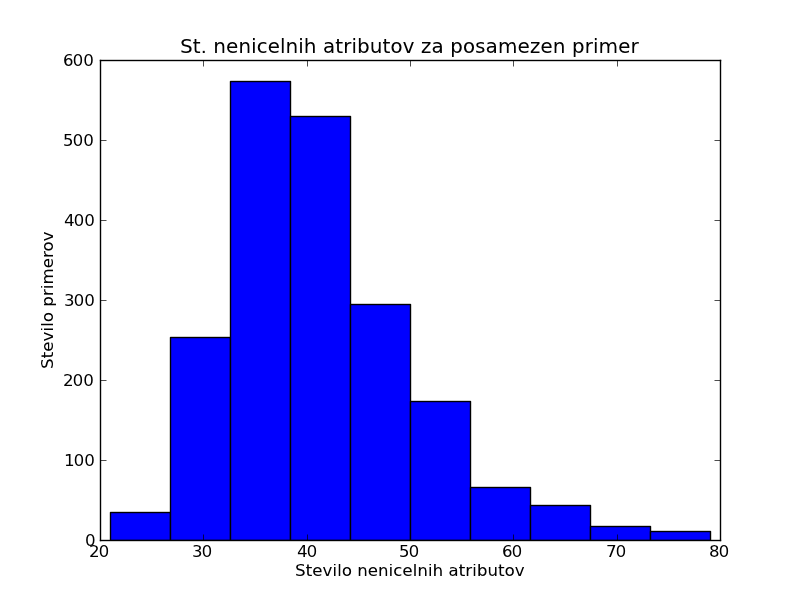
\includegraphics[scale=0.5]{examples.png}
%\caption{Prikaz atributov, ki imajo vrednost različno od 0 za posamezen primer}
%\label{primeri}
%\end{center}
%\end{figure}

\section{Izjava o izdelavi domače naloge}
Domačo nalogo in pripadajoče programe sem izdelal sam.
\end{document}
